
\usetikzlibrary{arrows.meta}
\tikzstyle{myarrows}=[line width=1mm,draw=blue,-triangle 45,postaction={draw, line width=3mm, shorten >=4mm, -}]
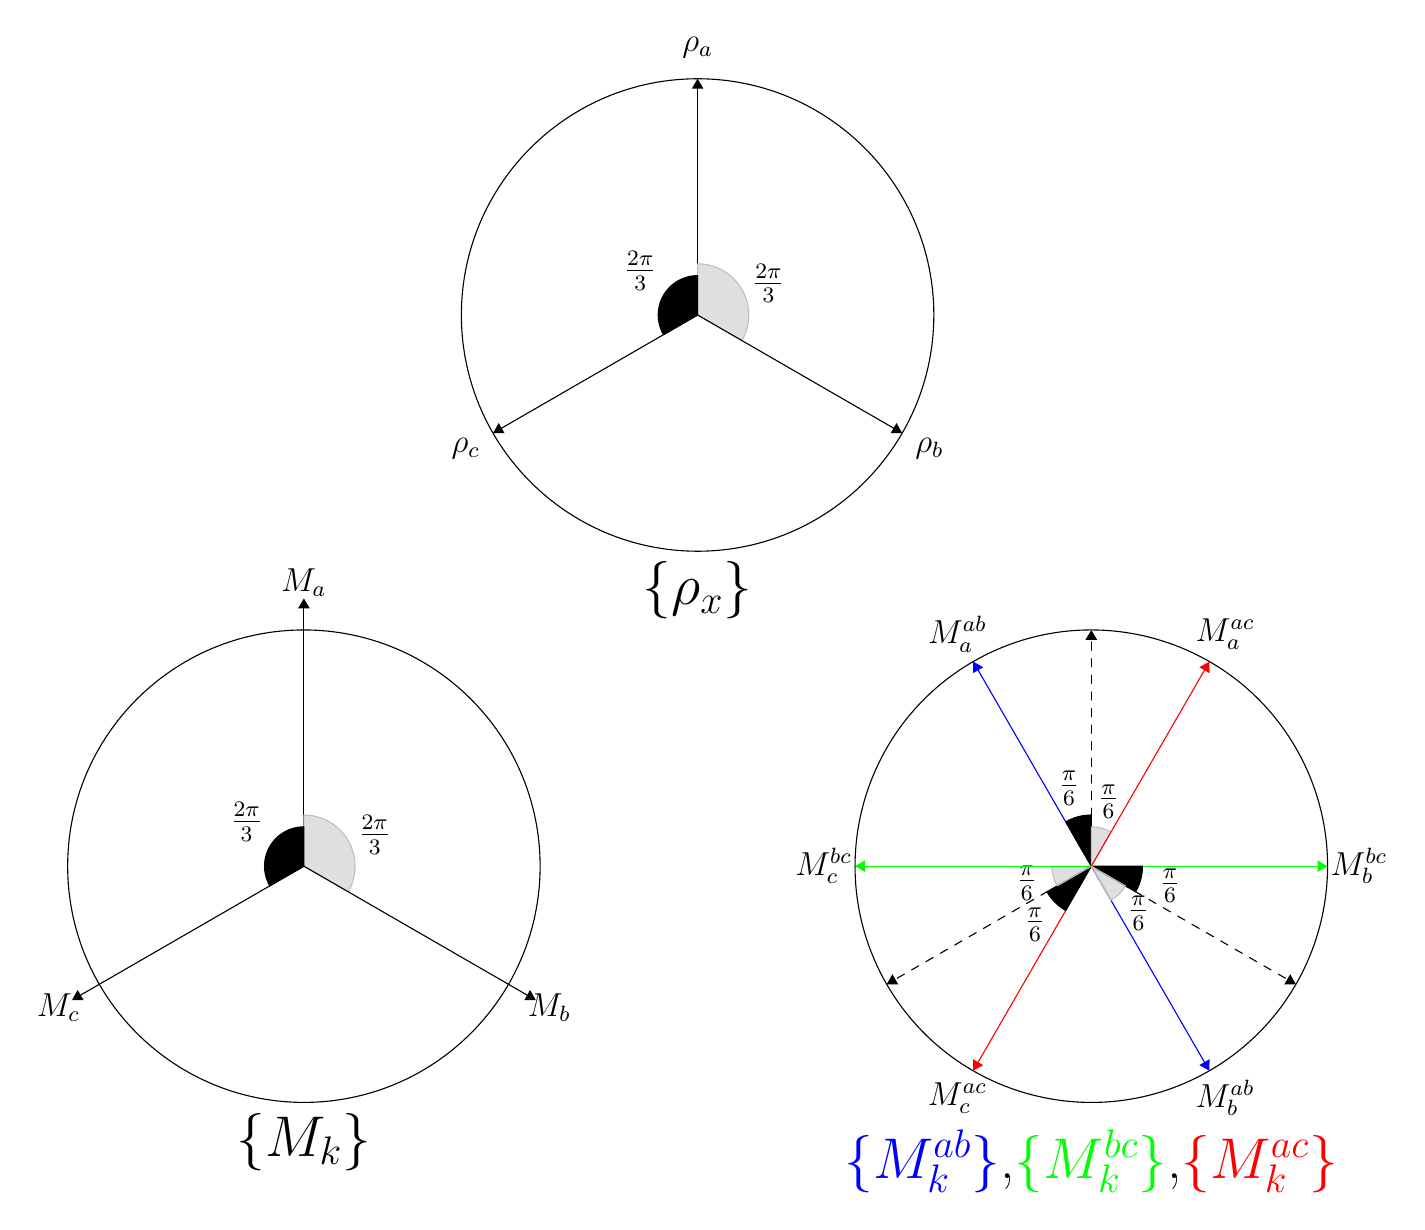
\begin{tikzpicture}[line cap=round, line join=round, >=Triangle]

\begin{scope}[ shift={(0,0)}]
\draw  (0,0) ellipse (3 and 3);


\draw[->]  (0,0) -- (0,3);
\draw (0,3.4) node {\large $\rho_a$};
\draw [shift={(0,0)},lightgray, fill, fill opacity=0.5] (0,0) -- (90:0.65) arc (90:-30:0.65) -- cycle;
\node at (0.9,0.4) {\large $\frac{2\pi}{3}$};

\begin{scope}[rotate=120]
    \draw[->]  (0,0) -- (0,3);
	\draw (0,3.4) node {\large $\rho_c$};
	
\draw [shift={(0,0)}, fill] (0,0) -- (90:0.5) arc (90:-30:0.5) -- cycle;
\node at (0.85,0.35) {\large $\frac{2\pi}{3}$};
\end{scope}

\begin{scope}[rotate=240]    
	\draw[->]  (0,0)  -- (0,3);
	\draw (0,3.4) node {\large $\rho_b$};
\end{scope}
\node at (0,-3.5) {\huge $\{\rho_x\}$ };
\end{scope}


\begin{scope}[ shift={(-5,-7)}]
\draw  (0,0) ellipse (3 and 3);


\draw[->]  (0,0) -- (0,3.4);
\draw (0,3.6) node {\large $M_{a}$};
\draw [shift={(0,0)}, lightgray, fill, fill opacity=0.5] (0,0) -- (90:0.65) arc (90:-30:0.65) -- cycle;
\node at (0.9,0.4) {\large $\frac{2\pi}{3}$};

\begin{scope}[rotate=120]
   \draw[->]  (0,0) -- (0,3.4);
\draw (0,3.6) node {\large $M_{c}$};
	
\draw [shift={(0,0)}, fill] (0,0) -- (90:0.5) arc (90:-30:0.5) -- cycle;\node at (0.85,0.35) {\large $\frac{2\pi}{3}$};
\end{scope}

\begin{scope}[rotate=240]    
	\draw[->]  (0,0) -- (0,3.4);
\draw (0,3.6) node {\large $M_{b}$};
\end{scope}
\node at (0,-3.5) {\huge $\{M_k\}$ };
\end{scope}


\begin{scope}[ shift={(5,-7)},rotate=30]
\draw  (0,0) ellipse (3 and 3);


\draw[->,color=blue]  (0,0) -- (0,3);
\draw[->,dashed,rotate=-30]  (0,0) -- (0,3);
\draw[->,color=blue]  (0,0) -- (0,-3);
\draw (0,3.4) node {\large $M^{ab}_a$};
\draw (0,-3.4) node {\large $M^{ab}_b$};
\draw [shift={(0,0)}, fill] (0,0) -- (90:0.65) arc (90:60:0.65) -- cycle;
\node at (0.6,0.6) {\large $\frac{\pi}{6}$};
\draw [shift={(0,0)}, lightgray, fill, fill opacity=0.5] (0,0) -- (60:0.5) arc (60:30:0.5) -- cycle;
\node at (0.25,1) {\large $\frac{\pi}{6}$};


\begin{scope}[rotate=120]
\draw[->,dashed,rotate=-30]  (0,0) -- (0,3);
    \draw[->,color=red]  (0,0) -- (0,3);
    \draw[->,color=red]  (0,0) -- (0,-3);
	\draw (0,3.4) node {\large $M^{ac}_c$};
	\draw (0,-3.4) node {\large $M^{ac}_a$};
	\draw [shift={(0,0)}, fill] (0,0) -- (90:0.65) arc (90:60:0.65) -- cycle;
\node at (0.6,0.6) {\large $\frac{\pi}{6}$};
\draw [shift={(0,0)}, lightgray, fill, fill opacity=0.5] (0,0) -- (60:0.5) arc (60:30:0.5) -- cycle;
\node at (0.25,1) {\large $\frac{\pi}{6}$};

\end{scope}

\begin{scope}[rotate=240]    
\draw[->,dashed,rotate=-30]  (0,0) -- (0,3);
	 \draw[->,color=green]  (0,0) -- (0,3);
    \draw[->,color=green]  (0,0) -- (0,-3);
	\draw (0,3.4) node {\large $M^{bc}_b$};
	\draw (0,-3.4) node {\large $M^{bc}_c$};
	\draw [shift={(0,0)}, fill] (0,0) -- (90:0.65) arc (90:60:0.65) -- cycle;
\node at (0.6,0.6) {\large $\frac{\pi}{6}$};
\draw [shift={(0,0)}, lightgray, fill, fill opacity=0.5] (0,0) -- (60:0.5) arc (60:30:0.5) -- cycle;
\node at (0.25,1) {\large $\frac{\pi}{6}$};
;
\end{scope}

\end{scope}

\node at (5,-10.75) {\huge {\color{blue} $\{M^{ab}_k\}$},{\color{green} $\{M^{bc}_k\}$},{\color{red} $\{M^{ac}_k\}$}};

\end{tikzpicture}